\documentclass[10pt,a4paper]{article}
\usepackage[utf8]{inputenc}
\usepackage[italian]{babel}
\usepackage{amsmath}
\usepackage{amsfonts}
\usepackage{amssymb}
\usepackage{graphicx}
\usepackage{siunitx}
\usepackage[left=2cm,right=2cm,top=2cm,bottom=2cm]{geometry}
\newcommand{\rem}[1]{[\emph{#1}]}
\newcommand{\exn}{\phantom{xxx}}
\usepackage[italian]{babel}
\usepackage[utf8]{inputenc}
\usepackage{siunitx}
\usepackage{graphicx}
\usepackage{xcolor}
\usepackage{amsfonts}
\usepackage{amsmath}
\usepackage{amsthm}
\usepackage{tikz}
\usepackage{pgfplots}
\usepackage{enumitem}
\usepackage{siunitx}
\date{\today}
\usetikzlibrary{shapes.geometric,calc,matrix,arrows,snakes,shapes,patterns}
\title{Esercitazione 10B: Caratteristiche porte logiche e semplici circuiti logici}
\author{Massimo Bilancioni, Alessandro Foligno}
\begin{document}	
\maketitle
	
	\section{Caratteristiche statiche}
	Si monta il circuito come in figura,, utilizzando resistenze con valori  $R_{2~nominale}=100\Omega $,~
	$R_{1~meas}\approx2.08\pm0.01 k \Omega$ è la resistenza massima del potenziometro che ci permette di variare la tensione in ingresso al componente (e quindi di mettere l'ingresso ad H/L).\\
	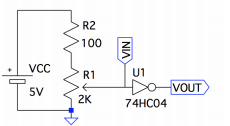
\includegraphics[scale=0.9]{Cattura.png}\centering
\\Si sono prese varie della tensione in ingresso/ uscita,  ottenute variando la posizione del potenziometro,e sono riportate nella seguente tabella. Si è poi tracciato un grafico $V_{in}/V_{out}$ con i dati raccolti. \\
	
	\begin{center}
\begin{tabular}{|c|c|c|c|}
	\hline 
	$V_{in}$ & $\sigma(V_{in})$ & $V_{out}$ & $\sigma(V_{out})$ \\ 
	\hline 
	0.04&0.06&5.0&0.1\\ \hline
	0.28&0.05&5.0&0.1\\ \hline
	0.6&0.07&5.0&0.1\\ \hline
	1.0&0.06&4.96&0.1\\ \hline
	1.06&0.06&4.7&0.1\\ \hline
	1.18&0.06&3.88&0.08\\ \hline
	1.27&0.07&2.92&0.08\\ \hline
	1.4&0.08&1.5&0.08\\ \hline
	1.4&0.08&1.08&0.08\\ \hline
	1.48&0.08&0.1&0.08\\ \hline
	1.9&0.08&0.09&0.08\\ \hline
	2.4&0.08&0.08&0.07\\ \hline
\end{tabular} 
	\end{center}
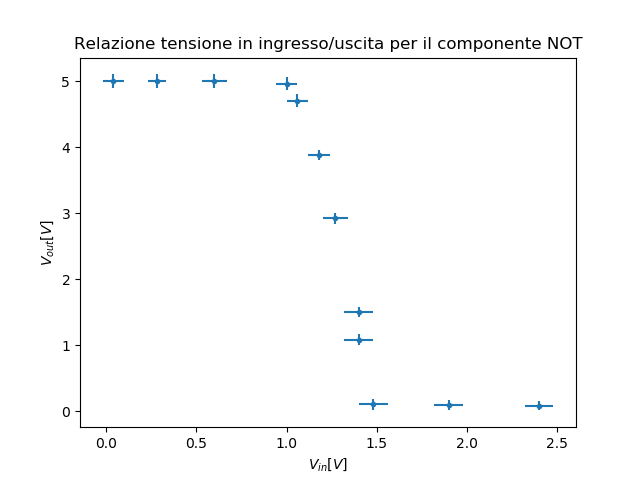
\includegraphics[scale=0.5]{gain.png}\centering
\\Come si può vedere, il comportamento del componente è quasi quello di una funzione a gradino, piuttosto piatta fino a un certo punto, e poi con una brusca variazione.
Osservando i punti del grafico dove inizia e finisce la variazione, posso stimare VIL, VOH  VIH, VOL , valori da confrontare con quelli sul datasheet.
\\Ottengo, come stima:
\begin{enumerate}
	\item $V_{IL}\approx0.9 V,~V_{IL~nominale}=0.7V$
	\item $V_{IH}		\approx 1.5V,~V_{IH~nominale}=2V$
	\item $V_{OL}\approx0.1V,~V_{OL~nominale}=0.5V$
	\item $V_{OH}\approx5V,~V_{OH~nominale}=2.5V$
\end{enumerate}

	\section{Caratteristiche dinamiche}
\textcolor{red}{correggere in base all'immagine l'ampiezza dell'onda quadra, aggiungere erroe ai tempi, confronto finale può essere colpa del generatore che non è abbastanza veloce a cambiare}
Abbiamo inviato un'onda quadra con valori  $0-5 \si{\volt}$ in ingresso. Nelle figure compaiono l'ingresso (arancio) e l'uscita (blu) rispettivamente negli istanti in cui l'ingresso passa da basso ad alto e da alto a basso.
Nel primo caso misuriamo $t_{PHL}= 20 \si{\nano\second}$ nel secondo  misuriamo $t_{PLH} = 40\si{\nano \second}$.
Nel datasheet sono riportati i valori tipici: $t_{PHL}= 10 \si{\nano\second}$, $t_{PLH} = 9\si{\nano \second}$ e quello massimo $t_{PHL}^{MAX}= t_{PLH}^{MAX}= 15 \si{\nano\second}$.


\section{Costruzione di circuiti logici elementari}
Si è verificato il comportamento della porta NAND tramite il led e l'interruttore con il circuito mostrato in \textcolor{red}{figura}.

Il circuito AND è stato costruito con due porte NAND secondo lo schema mostrato in Figura (\ref{fig:and}).

\begin{figure}
			\centering
			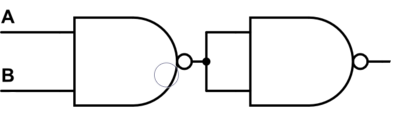
\includegraphics[scale=0.60]{and}
			\caption{schema porta AND}
			\label{fig:and}
\end{figure}
Per il circuito OR  si sono usate tre porte NAND, Figura (\ref{fig:or}).
\begin{figure}
			\centering
			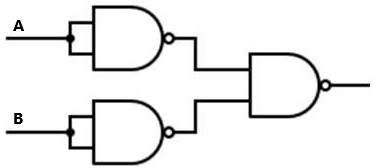
\includegraphics[scale=0.85]{or}
			\caption{schema porta OR}
			\label{fig:or}
\end{figure}
Il circuito XOR  è stato realizzato con quattro porte NAND, Figura (\ref{fig:xor}).
\begin{figure}
			\centering
			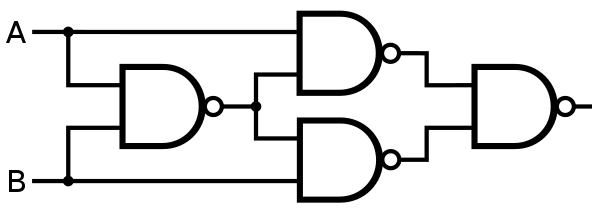
\includegraphics[scale=0.55]{xor}
			\caption{schema porta XOR}
			\label{fig:xor}
\end{figure}
Il sommatore a due bit è stato costruito con cinque porte NAND: una in meno rispetto alla somma AND $+$  XOR perchè una porta era in comune, Figura (\ref{fig:som}).
\begin{figure}
			\centering
			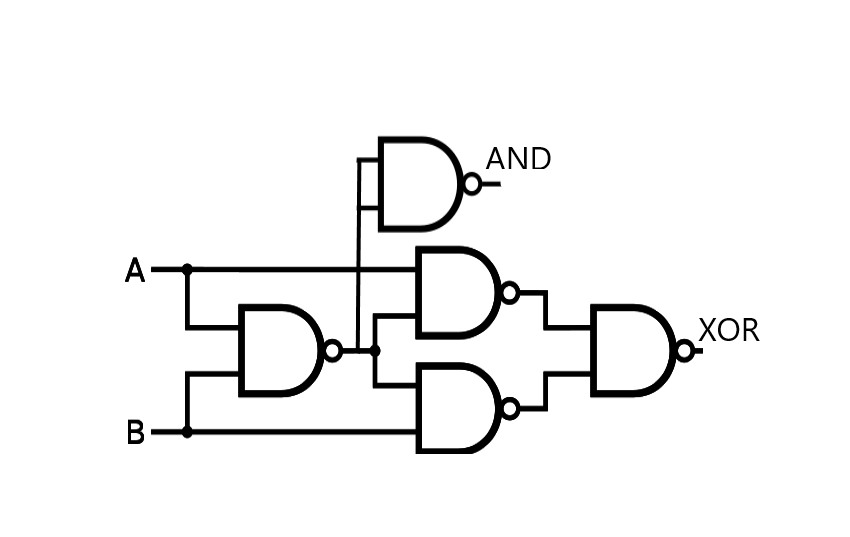
\includegraphics[scale=0.55]{sommatore}
			\caption{schema sommatore a due bit}
			\label{fig:som}
\end{figure}

Si sono verificati i comportamenti  previsti tramite l'accensione o meno del led  (due nel caso del sommatore a due bit) per tutte le configurazioni degli interruttori (due nel caso del sommatore a due bit).


\end{document}